\chapter{Consensus protocol example}
\label{app:consensus-example}

\begin{figure}[htb]
    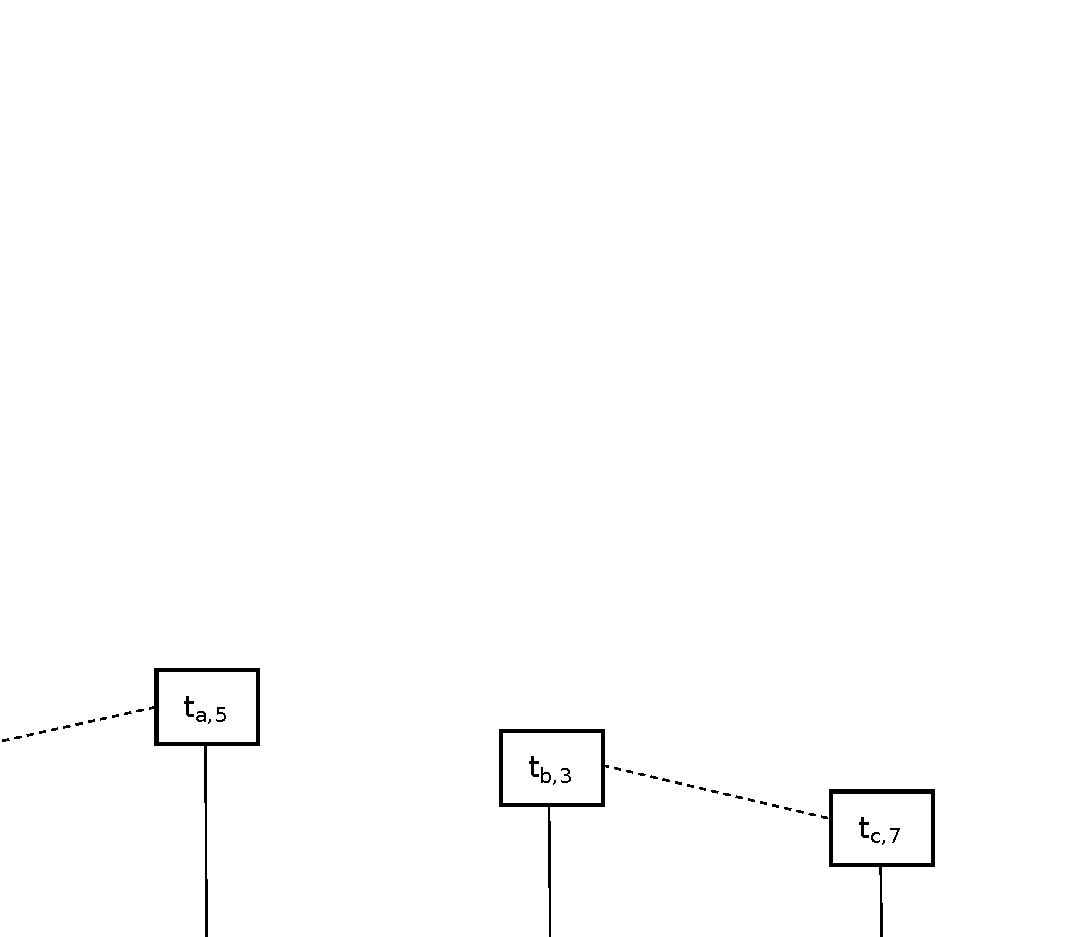
\includegraphics[trim={0 0 0 11cm}, clip, width=1.0\textwidth]{trustchain-1}
    \centering
    \caption{We begin in a state where some facilitators $\F_{r-2}$ just agreed on the consensus result $\C_{r-1}$ but have not yet propogated it yet.}
    \label{fig:trustchain-1}
\end{figure}

\begin{figure}[htb]
    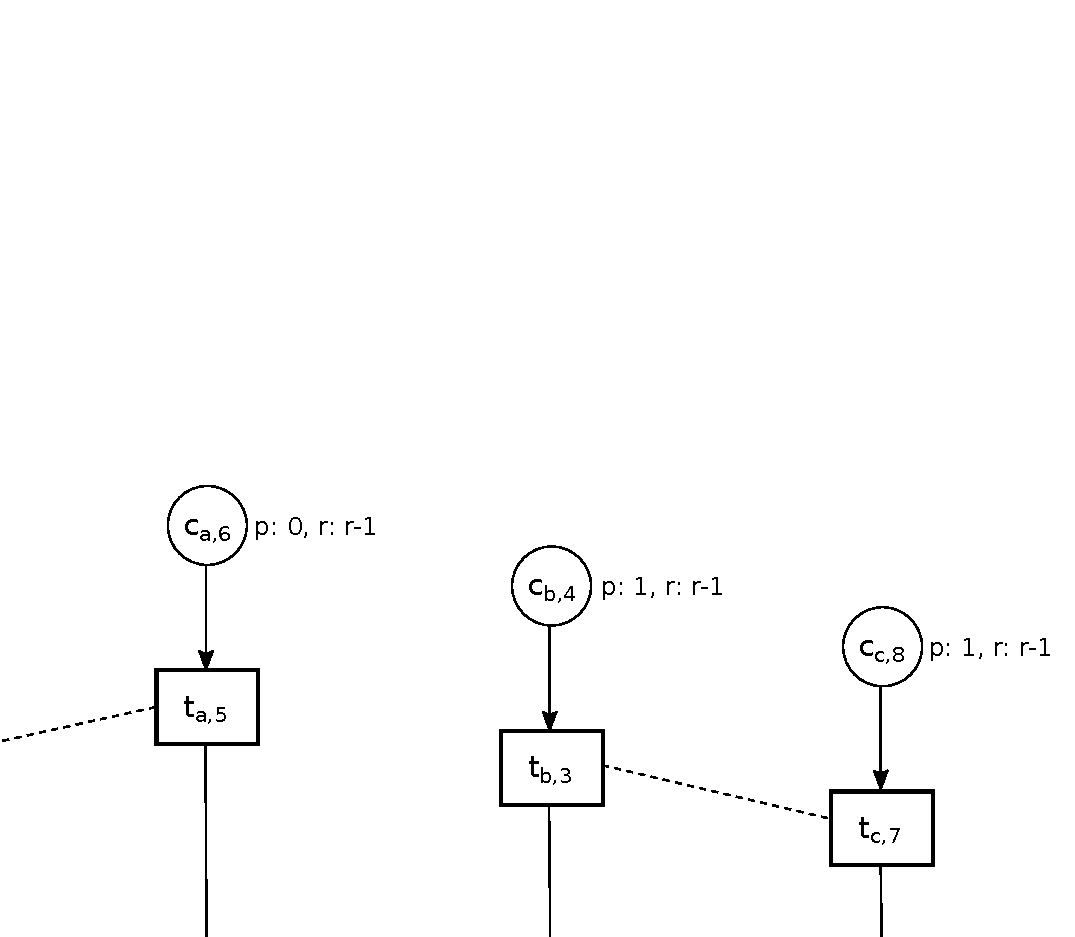
\includegraphics[trim={0 0 0 8cm}, clip, width=1.0\textwidth]{trustchain-2}
    \centering
    \caption{The facilitators propogates $\C_{r-1}$. Upon receiving it, the nodes perform two tasks;
    (1) elect new facilitators $\F_{r-1}$ by selecting the first $n$ nodes ordered by $\textsf{H}(\C_{r-1} || pk)$,
    and (2) create new CP blocks---$c_{a, 6}, c_{b, 4}$ and $c_{c, 8}$.
    $\textsf{H}(\cdot)$ is a cryptographically secure hash function and $pk$ is the public key of the respective node.}
    \label{fig:trustchain-2}
\end{figure}

\begin{figure}
    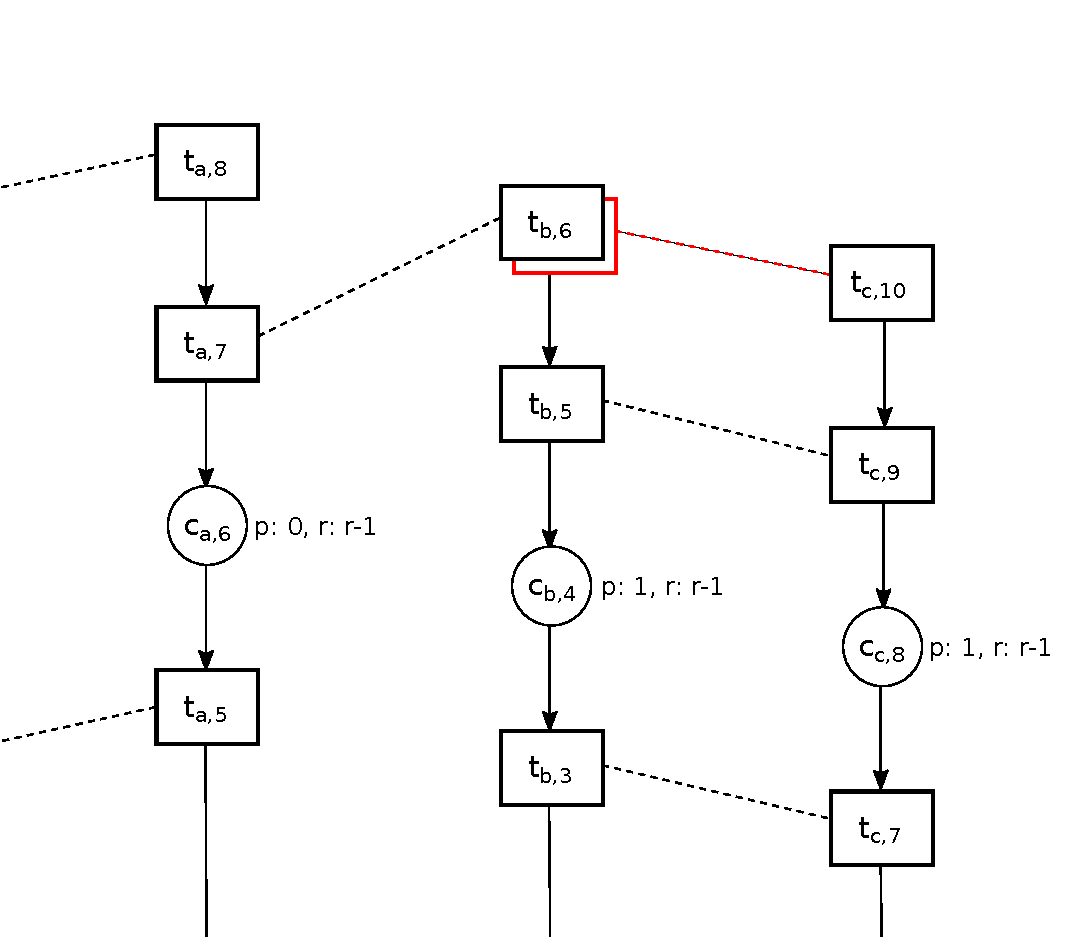
\includegraphics[trim={0 0 0 2cm}, clip, width=1.0\textwidth]{trustchain-3}
    \centering
    \caption{Nodes now send their new CP blocks to the new facilitators $\F_{r-1}$.
    While $\F_{r-1}$ is trying to reach consensus on a set of CP blocks,
    nodes carry on making transactions as usual (concurrently).
    We remark that the to-be-agreed consensus result $\C_r$ is created using CP blocks from the previous round---$c_{a, 6}, c_{b, 4}$ and $c_{c, 8}$.
    }
    \label{fig:trustchain-3}
\end{figure}

\begin{figure}
    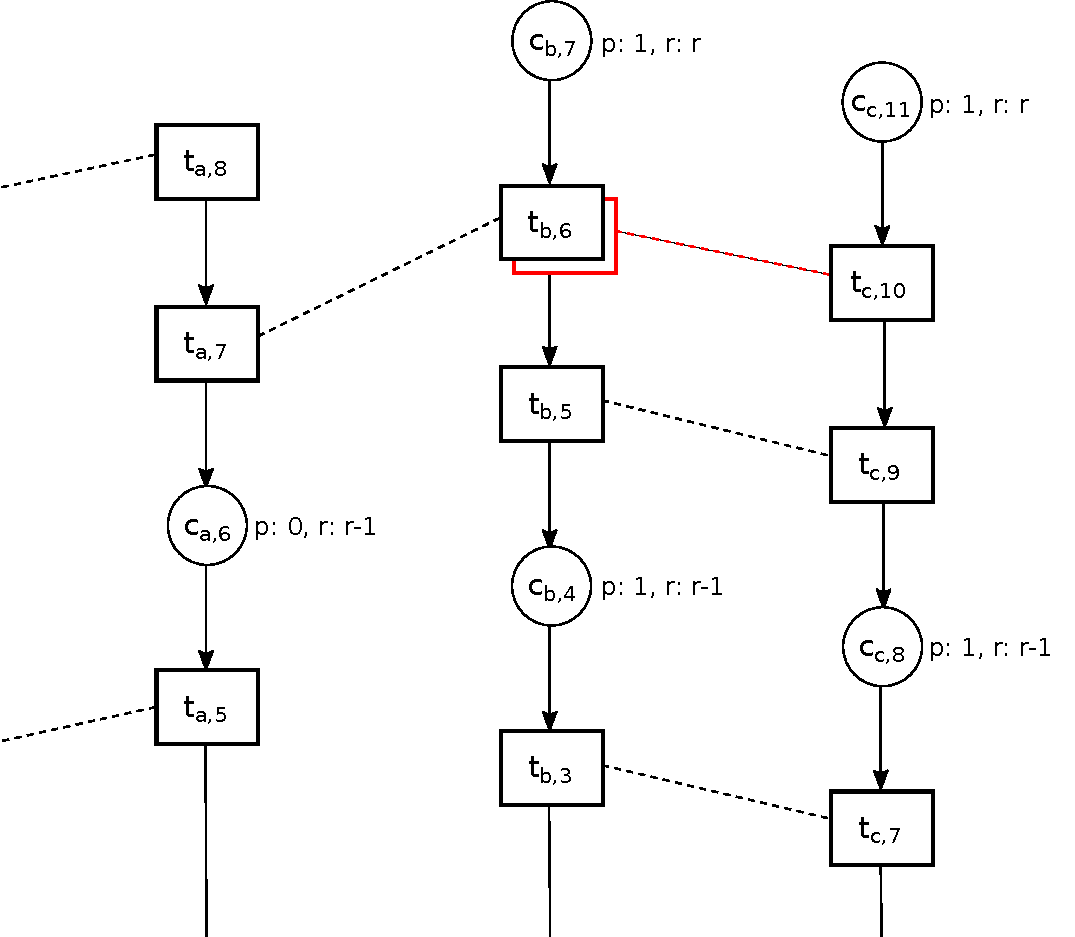
\includegraphics[width=1.0\textwidth]{trustchain-4}
    \centering
    \caption{Finally, when $\F_{r-1}$ decides on $\C_r$ (which should contain $c_{a, 6}, c_{b, 4}$ and $c_{c, 8}$) and disseminates it.
    Nodes compute new facilitators $\F_{r}$ and create new CP blocks.}
    \label{fig:trustchain-4}
\end{figure}